\documentclass[12pt, a4paper, dutch]{article}
\usepackage[margin=1in]{geometry}

\usepackage{float}
\usepackage{babel}
\usepackage{siunitx}
\usepackage{amsmath}
\usepackage{csquotes}
\usepackage{parskip}
\usepackage{unicode-math}
\usepackage{fontspec}
\usepackage{tabularx}
\usepackage{booktabs}
\usepackage{needspace}
\usepackage{hyperref}
\usepackage{graphicx}
% \usepackage[backend=biber,
% 	bibencoding=utf8,
% 	style=apa
% ]{biblatex}

\setmainfont{TeX Gyre Schola}
\setmathfont{TeX Gyre Schola Math}
\sisetup{
	group-separator = {.},
	output-decimal-marker = {,}
}

\bigskipamount=7mm
\medskipamount=4mm
\parindent=0mm

\begin{document}
Ontwerpdocument \hfill \textbf{Loek Le Blansch (2180996)}\\
Project Stylofoon \hfill \today
\medskip

In dit document staan alle ontwerpfasen van de stylofoon met eventuele verklaring van
ontwerpkeuzes. Aan het einde van dit document zitten kopieën van het elektrisch
schema en PCB ontwerp op ware grootte.

\section{Ontwerpschets}

\begin{figure}[H]
	\centering
	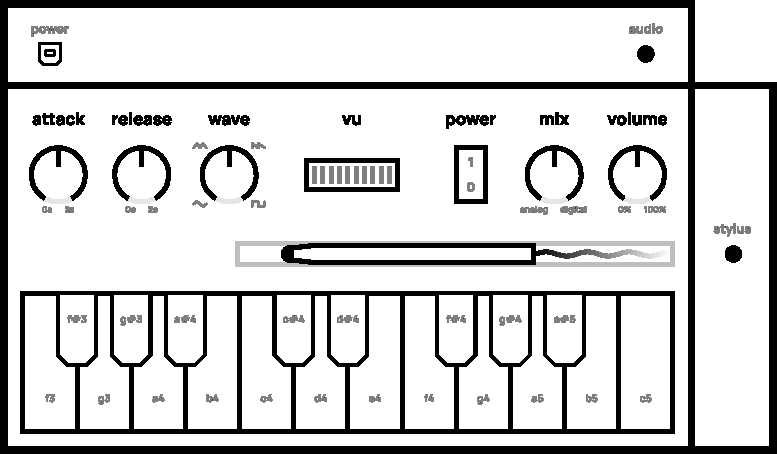
\includegraphics{figs/case-layout-sketch.pdf}
	\caption{Schets van de knoppenlayout op de voor-, zij- en bovenkant}
\end{figure}

Voor de stylofoon wou ik graag dat alle in- en outputs naast het keyboard zelf op een
regel zouden liggen. Zo zou het makkelijk zijn om de status van het hele instrument
in \'e\'en oogopslag te zien. Ook is er een losse voedingsaansluiting aan de
bovenkant, en een tweede 3.5mm jack om de stylus los te kunnen koppelen.

\newpage
\section{Blokschema}

\begin{figure}[H]
	\centering
	\includegraphics{figs/stylofoon blokschema-top-level.pdf}
	\caption{Blokschema (niveau 1)}
\end{figure}

\begin{figure}[H]
	\centering
	\includegraphics[width=\textwidth]{figs/stylofoon blokschema-level 2.pdf}
	\caption{Blokschema (niveau 2)}
\end{figure}

\newpage
\section{Elektrisch schema}

\begin{figure}[H]
	\centering
	\includegraphics[
		width=\textwidth,
		clip,
		trim=19.7mm 74mm 19mm 12mm,
	]{figs/eschema.pdf}
	\caption{Elektrisch schema}
\end{figure}

Voor de `555 vco' (555 voltage-controlled oscillator) is een minder gebruikelijke
opstelling van de 555 timer te zien. Ik heb voor deze opstelling gekozen omdat ik van
plan was de Arduino te gebruiken om uit te lezen welke toets er wordt gespeeld. Met
de aanbevolen opstelling uit de projectlessen werd een variabele weerstand gebruikt
om de toonhoogte die de 555 osillator produceert te veranderen, en dit zou het meten
met de Arduino lastig maken.

De weerstandswaardes voor de weerstandsladder zijn uitgerekend door eerst met een
oscilloscoop en de 555 opstelling op een breadboard de juiste spanningen voor de
benodigde frequenties te vinden. Vervolgens heb ik een spreadsheet programma gebruikt
om uit te rekenen waar deze spanningen vallen tussen 0 en 5V (vcc). Daarna heb ik een
totale weerstandswaarde van 50\si{\kilo\ohm} gekozen voor de weerstandsladder, en het
spreadsheet programma laten uitrekenen hoe groot de weerstanden tussen de toetsen
moeten zijn. Daarna heb ik een programma geschreven die de uitgerekende
weerstandswaardes van de spreadsheet opdeelt in weerstanden die in het techlab
beschikbaar zijn.

Voor de rest zijn de LM386 audio versterker opstelling en de LM3914 vu-meter
opstelling gelijk aan de aanbevolen toepassing uit hun datasheets, met als enige
uitzondering de toegevoegde peak detector van de vu-meter.

\section{PCB ontwerp}

\begin{figure}[H]
	\centering
	\includegraphics[
		width=\textwidth,
		clip,
		trim=19.7mm 81mm 122mm 15mm,
	]{figs/pcb.pdf}
	\caption{PCB ontwerp. Rood is voorkant, blauw is achterkant}
\end{figure}

Voor het PCB ontwerp heb ik geprobeerd kleine componenten (diode's, weerstanden en
keramische condensatoren) zo dicht mogelijk op de chips te plaatsen, zodat het
makkelijker zou zijn om lange lijnen te trekken over de rest van de printplaat zonder
te veel via's te gebruiken. Ook heb ik extra jumper headers toegevoegd zodat ik
metingen en nog eventuele correcties zou kunnen maken na de hand.

\end{document}

